\subsection{Model Accuracy}
\begin{figure*}
    \centering
    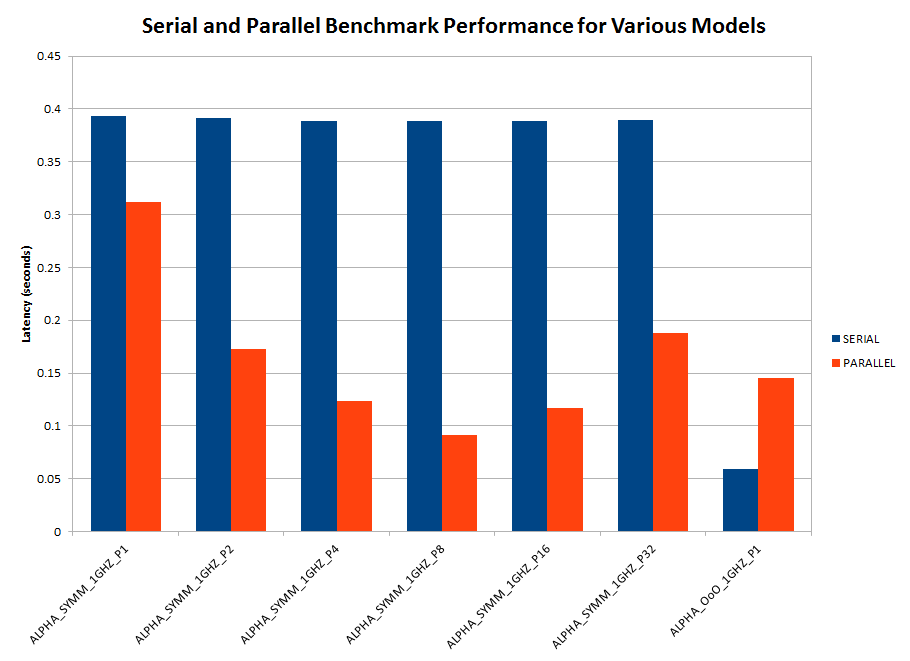
\includegraphics[scale=0.8]{../images/SerialParallelBenchmarks-Latency.png}
    \caption{The serial and parallel models perform appropriately and accurately for different benchmarks (P16 refers to 16 cores)}
    \label{fig:serialparallel}
\end{figure*}
\begin{figure*}
    \centering
    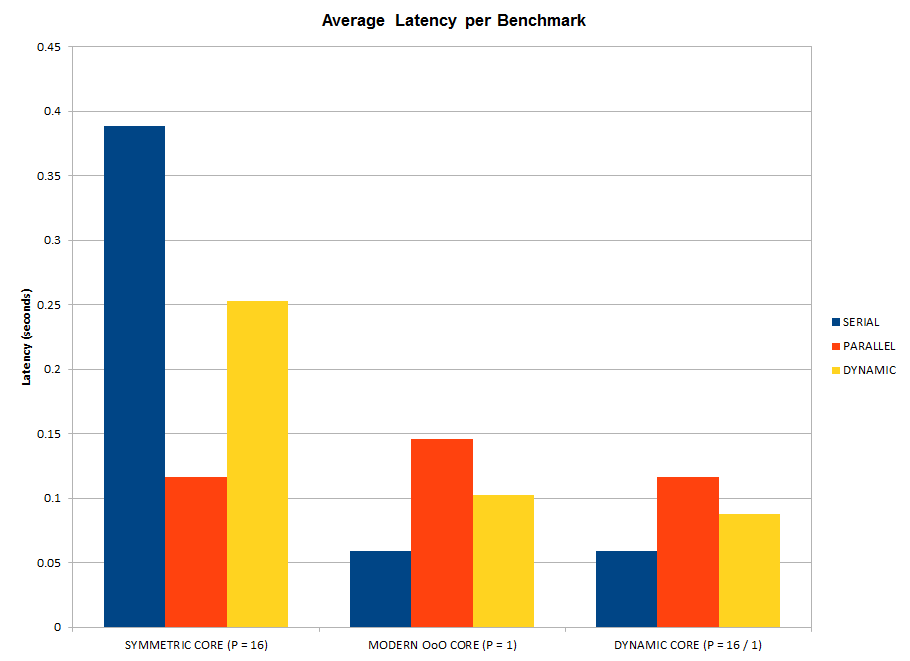
\includegraphics[scale=0.8]{../images/DynamicBenchmark-Latency-16.png}
    \caption{A dynamic core performs better than a 16 symmetric multicore machine and a single modern out-of-order machine}
    \label{fig:dynamic}
\end{figure*}
\begin{figure*}
    \centering
    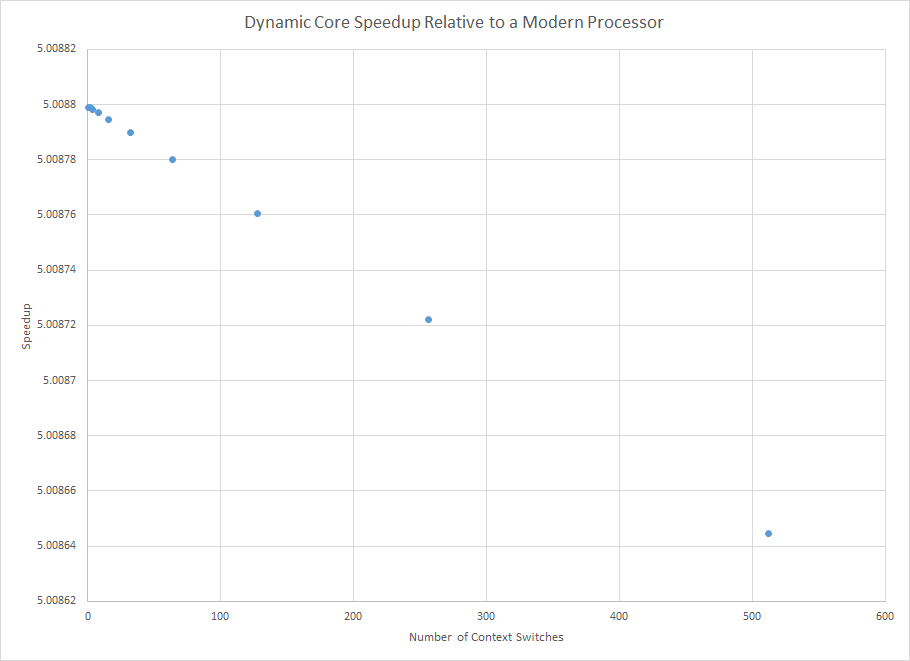
\includegraphics[scale=0.8]{../images/Switching.png}
    \caption{Fine granurality switching degrades performance gains}
    \label{fig:switch}
\end{figure*}
\begin{figure*}
    \centering
    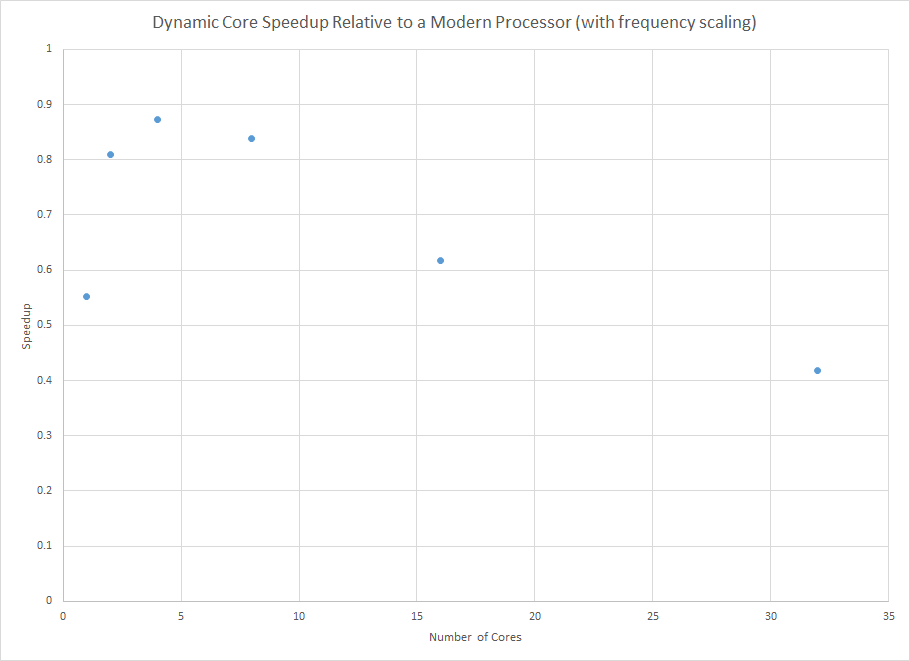
\includegraphics[scale=0.8]{../images/FrequencyScaling.png}
    \caption{Increasing the number of cores scales down the serial model frequency, resulting in a peak performance at four cores}
    \label{fig:frequency}
\end{figure*}
First, we needed to verify that our serial and parallel models were accurate. As expected, the serial model out performed the parallel model at serial tasks. Additionally, the parallel model performed the same for a serial task regardless of the number of cores; this is expected, since only a single core can effectively be used. Finally, the parallel model performed better that the serial model for parallel programs. However, it is worth noting that as the number of cores increased passed eight, the parallel performance began to degrade. At 32 cores, the performance was even worse than the serial model. Even so, we feel that these models are accurate for our theoretical study. See Figure \ref{fig:serialparallel} for these results.

\subsection{Is Dynamic Better?}
Ultimately, we wanted to answer the question ``Is Dynamic Better?''. At this stage, ``better'' is simply evaluated in terms of performance (we will go into more detail later). As can be seen in Figure \ref{fig:dynamic}, a dynamic core performs better in terms of average latency over the dynamic benchmark. Based on these results, the dynamic core has about a 4x improvement over a single baseline core machine (a basline core being the cores used to make up the parallel model), a 2.9x improvement over a sixteen core symmetric multicore machine, and 1.2x improvement over a modern, out-of-order processor. Note that we assumed the TimingSimple model in gem5 was sufficient to be used as our baseline core. This conclusion is corroborated by the results in Figure \ref{fig:serialparallel}; yet, if we had used a RISC pipelined architecture instead of a single cycle processor, the parallel model performance would have been even better (note how small the difference is between the parallel model and the serial model for the parallel benchmark in Figure \ref{fig:dynamic}). So, if anything, our dynamic core would have even greater performance gains.

However, as we briefly mentioned before, ``better'' is more than just performance. Especially on a mobile device, ``better'' is determined by efficiency. While we did not quantitatively determine the power consumption, we can qualitatively say a dynamic core will be more power efficient by nature. Since the symmetric multicore is made up of small, low power cores, and these same cores make up the basis for a dynamic core, a dynamic core is bound to be power efficient. There is, of course, overhead associated with a dynamic core. But this overhead should be no more than the overhead involved in a modern, out-of-order processor. We can analytically estimate this power overhead. Based on research at MIT, the maximum total power for a flip-flop or latch in a high performance system is 350 uW. Given that we are simulating an eight issue-width modern, out-of-order processor, we can expect about eight functional units (functional units scale with issue width). Since each function unit requires two inputs and one output (32-bits each) to be muxed, each functional unit will have $(3 muxes) \dot ((32 latches) + (32 flip-flops)) = 192 latches/flip-flops$. So, the average power overhead is $0.350(8)(192) = 537.6$ mW, which is minimal compared to the power consumption of a modern, out-of-order processor. So, speculatively (with some evidence), we can say that a dynamic core should consume less power than a modern, out-of-order processor, while still performing better.

\subsection{Peak Number of Switches}
When discussing a processor that performs context switching, it is useful to mention granurality. In other words, how often should a processor be switching between serial and parallel mode. As Figure \ref{fig:switch} shows, the finer grained the context switching, the lower the performance gains. Do not let the scale of the graph be misleading, the problem has purposefully been scaled up. So, our smallest building block between a context switch is a full program long (i.e. a full FFT or voice compression algorithm). Thus, the degradation is not as drastic numerically. However, logically, the trend should hold as the granularity becomes finer. Since the only factor degrading the performance is a linear constant for the interconnect latency, it follows that very fine grained switching will lower performance gains visibly.

\subsection{Frequency Scaling}
Though increasing the cores in a dynamic processor will result in performance gains due the to the parallel mode running faster, the serial portion will begin to suffer. A large number of cores means a greater area, which mean a longer critical path for the serial model. Based of off Pythagorean's theorem, we hypothesized that as the number of cores increased, the frequency would scale on the order of $1 / \sqrt{n}$. After re-running our original tests, we determined the new dynamic core latencies with a scaled frequency serial model. The speedup relative to a 1 GHz modern, out-of-order core can be seen in Figure \ref{fig:frequency}. There is a peak performance gain at four cores, before the speedup decays. So, while a dynamic core is better in an ideal sense, when practical constraints are applied to it, performance begins to degrade.

\subsection{Practicality}
In addition to our theoretical models, we chose to compare our dynamic core to modern, out-of-order, dual core processor, which is typical for the average device today. The speedup was 0.75x, so a decrease in performance. One arguement in favor of a dynamic core might be that a dual core, eigth issue width, out-of-order processor is equivalent to a single sixteen issue width out-of-order processor when we convert it to a serial model. We considered this, but noticed little improvement between a serial model using an eight issue width core and a sixteen issue width core.